\documentclass{article}
\def\npart {2}
\def\nterm {LMS Summer School}
\def\nyear {2021}
\def\nlecturer {Vanya Cheltsov}
\def\ncourse {Geometry of nets of conics}

\input{header}

\begin{document}
  \maketitle

\textbf{Suggested Reading} - Miles Reid, Undergrad Algebraic Geometry, contains other book recommended. Harris. Coxeter. Harsher, Shafarevich, Methods of Algebraic Geometry - Hodge, Ideals, Varieties and Algorithms.\\

\section{Overview}
This course is an introduction to Projective Geometry. In L3cture 1, we will consider and define the complex projective plane and lines in it, define projective transformations and their properties and finally Sylvester-Galllai Theorem.

\subsection{What is a line?}
In Algebraic Geometry we can use algebra, but it comes dry and we lose a geometric intuition.
\begin{figure}[!ht]
\centering
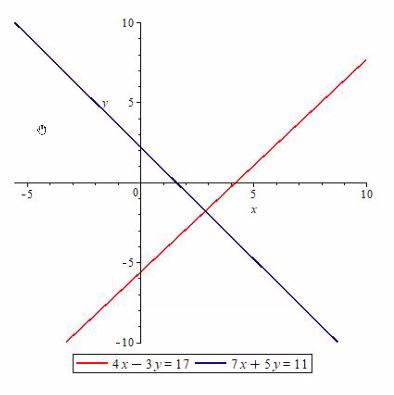
\includegraphics{./figures/L1.1}
\caption{This shows two lines intersect at one point}
\end{figure}

This picture is real, which is no good for us. Reals aren't algebraically closed, which create lots of problems and holes. If we look at the Cremona Group, theres a theorem about generators of this group, if we consider the reals, this is a really new result. Reals makes the problem too difficult and so we consider the complexes to make everything so much simpler.\\

\begin{ndefi}[Line]
  A line in $\C^2$ is a subset that is given by,
  $$ ax + by + c = 0 $$
  for some $a, b, c \in \C$ such that $(a, b) \ne (0, 0)$
\end{ndefi}

and here is a lemma,
\begin{nlemma}[]
  There is a unique line in $\C$ for rach two distinct points.
\end{nlemma}
\begin{proof}
  Trivial by linear algebra
\end{proof}

\begin{nlemma}[]
  Suppose that $L_1 \ne L_2$ then $L_1 \cap L_2$ contains at least one point.
\end{nlemma}
\begin{proof}[]
  If $a_1b_2 - a_2b_1 \ne 0$, then $L_1 \cap L_2$ consists of a point,
  % $$ \left( \frac{b_2c_2}{a} \right) $$
\end{proof}

This is what Algebraic Geometry removes.

\subparagraph{What is a plane}
For us a plane is just $\R^2$, but complex plane is also not perfect. If you don't travel over the plane that far, you are OK, but if you do, you get global problems. Take travelling the globe as an example. We can call a sphere a plane, if we wish, locally, we do, we have a plane, but global questions have a problem, the earth isn't a plane\footnote{Sorry, flat eathers}.\\


When we talk about spaces, Algebraic Geometers mean a projective plane.

\begin{ndefi}[Projective Plane]
  Let $(x, y, z) \in \C^3$ st $(x, y, z) \ne (0, 0, 0)$ and let $[x : y : z]$ be a subset of $\C^3$ such that,
  $$ (a, b, c) \in [x : y : z] \iff \begin{cases}
    a = \l x\\
    b = \l y\\
    c = \l z
  \end{cases} $$
  for some non-zero complex $\l$
\end{ndefi}

\begin{ndefi}[]
  The projective place $\P^2_\C$ is the set of all possible $[x : y : z]$
\end{ndefi}

We refer to $\P_\C^2$ as points and we can say that,
$$ [1 : 2 : 3] = [7 : 14 : 21] = [2 - i : 4 - 4i : 3 - 3i] $$
and
$$ [1 : 2 : 3] \ne [3 : 2 : 1] $$
and
$$ [0 : 0 : 1] \ne [0 : 1 : 0] $$

\begin{remark}
 There is no point $[0 : 0 : 0]$
\end{remark}

\subsection{How to live in projective plane}
Let $U_z$ be the projective plane $\pc$ consisting of points $[x : y: z]$ with $z \ne 0$,

\begin{nlemma}[]
  The map $U_z \to \C$,
  $$ [x : y: z] = \left[\frac{x}{z} : \frac{y}{z} : 1\right] \mapsto (\frac{x}{z}, \frac{y}{z}) $$
  is a bijection.
\end{nlemma}
Thus we can identify $U_z = \C^2$, we call these charts and affine charts. These are exactly manifolds are we have three affine charts.

\begin{itemize}
  \item Put $\overline x = \frac{x}{z}$ and $\overline y = \frac{y}{z}$
  \item Then we can consider $overline
  x$ and $\overline y$ coordinates on $U_z = \C62$
\end{itemize}

\begin{question}
  What is $\pc \setminus U_z$
\end{question}
\begin{itemize}
  \item The subset $\pc$ consisting of points $[ x : y : 0]$
  \item We can identify this as $\P_\C^1$
\end{itemize}
If a question isnt homogenous, it doesnt make sense to do it in $\pc$. This is the same as it is for Linear Algebra.

\begin{ndefi}[Line]
  A line in $\pc$ is the subset given by,
  $$ Ax + By + Cz = 0 $$
  for some fixed point $[A : B : C] \in \pc$
\end{ndefi}
We sometimes call $\pc$ the dual plane here. We have polynomials of degree one.

\begin{eg}
  Let $P = [5 : 0 : 2]$ and $Q = [1:-1:1]$. Then,
  $$ 2x - 3y + 5z = 0 $$
  is the unique line
\end{eg}

\begin{eg}
  Let L be give by,
  $$ x + 2y + 3z = 0 $$
  Let $L'$ be $x - y =0$, we then have $L \cap L' = [1 : -1 : 0]$
\end{eg}

\begin{nthm}[]
  There is a unique line in $\pc$ that contains $P$ and $Q$
\end{nthm}

\begin{proof}[]
  Let $L$ be a line in $\pc$ that is given by $Ax + By + Cz = 0$, then take two different lines, solve the system and by rank-nullity implies that $L$ exists and is unique
\end{proof}

\begin{nthm}[]
  The intersections $L \cap L'$ consirst of one point in $\pc$
\end{nthm}
\begin{proof}
  The same as above.
\end{proof}

It's very easy to find intersections and lines theough two points, but we can use python to do it. We can also use a determinant formula,
$$ \det \begin{pmatrix}
11 & -7 & 1\\
2 & 5 & 1\\
x & y & z
\end{pmatrix} $$

\subsection{Parallel Lines? Do they meet?}
In classical geometry, this is at infinity. We can do this in agebra,\\

Let $U_z$ be the complement of $\pc$ to the line$z= 0$. Idenity,
$$ U_z = \C $$
with coordinates $\overline x = \frac{x}{z}$ and $y = \frac{y}{z}$

\begin{itemize}
  \item Let $\overline L = 2\overline x + 3\overline y + 5 = 0$
  \item Let $\overline L = 2\overline x + 3\overline y + 7 = 0$
  \item $L \cap L' = \varnothing$
\end{itemize}

\begin{question}
  Where do $\overline L$ and $\overline L'$
\end{question}

\subsection{Projective Transformations}
If we have an equation that can be simplified using some sort of change of variables. Let $\mathbf{M} \in M_{3\times 3}$ and $\phi : \pc \to \pc$ be given by,
$$ [x : y : z] = M \mathbf{x} $$
where $\mathbf{x}$ is just the vector formed of $x$. This is called the automorphism of $\pc$, but we dont have $[0 : 0 : 0]$, this is a problem as $\phi$ may output it, if $\mathbf{x}$ is in the kernel.

\begin{question}
  When $\phi$ well defined?
\end{question}
This is when $M$ is invertible or $\det M \ne 0$

\begin{ndefi}[Projective Transformation]
  If $\det M \ne 0$ we say that $\phi$ is a projective transformation.
\end{ndefi}

\subsection{Group of transformations}

Projective transformations of $\pc$ form a group.
\begin{itemize}
  \item Let $M$ be a atric in $GL_3(\C)$
  \item Denote by $\phi_M$ the corresponding projective transformation.
\end{itemize}

\begin{question}
  When $\phi_M$ is an idenity map?
\end{question}

The map $\phi_M$ is said to be the indentity $\iff$ $M$ is a scalar.

\begin{ndefi}[]
  We call $M$ is said to be scalar if $M$ is diagonal
\end{ndefi}

\begin{ncor}
   Let $G$  be a subgroup in $GL_3(\C)$ consistong of scalar matrices. The group of projective transformations of $\pc$ is isomorphic to,
   $$ PGL_3(\C) = GL_3(\C)\/G $$
\end{ncor}

We can look at mobius transformations, but for our plane. If you have four points in the plane, such that no three points are not collinear. Then there is a projective plane such that $\pc \to \pc$ such that,
$$ [1:0:0], [0:1:0], [0:0:1], [1:1:1] $$
so we let, $P_1 = [a_{11} : a_{12} : a_{13}]$ and $P_2 = [a_{21} : a_{22} : a_{23}]$ and $P_3 = [a_{31} : a_{32} : a_{33}]$ and then do $\phi$ on them and then it will map the basic points to ir points and so do the inverse. Let $\psi$ be $\phi$ and then apply it and then forma projective transformation and done.

\subsection{Sylvester - Gallai Problem}
\begin{problem}
  Let $\Sigma$ be the finite subset in $\R^2$. show that either $\Sigma$ is contained in one line, or there is a line containing exactly two points in $\Sigma$.
\end{problem}
\begin{itemize}
  \item This problem was proposed by Sylvester in 1893
  \item It was solved by Gallai in 1944
  \item A simpler proof was given by Kelly in 1948
\end{itemize}

Sylvester was not just a Geometry, he was interested in Algebra aswell, he worked with Complexes and he knew the problem was wrong. He knew a very simpler counter example.\\

\subsection{Hesse Configurations}


\begin{itemize}
  \item Nine points were the counterexample
  \item There are 12 lines passing through 2 points among them
  \item Each such line contain 3 points among nine.
\end{itemize}

\begin{figure}[!ht]
\centering
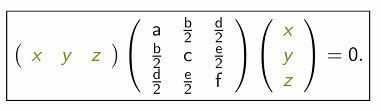
\includegraphics{./figures/L2.1}
\end{figure}

\begin{itemize}
  \item Let $\F$ be a field
  \item Let $\Sigma$ be a finite subset in $\P_\F^2$
\end{itemize}

Suppose that the subset $\Sigma$ is not contained in one line,

\begin{nlemma}[]
  There exists a line in $\P_\F^2$ contaning exactly two points in $\Sigma$,
  \begin{itemize}
    \item where $|\Sigma| \le 6$
    \item where $|\Sigma| = 7$ and $2 \ne 0$ in $\F$
    \item where $|\Sigma| = 8$
  \end{itemize}
\end{nlemma}

\begin{nthm}[]
  Suppose $|\Sigma| = 9$ and $\F=\C$. If there exists no line containing exactly two points of the set
\end{nthm}

\section{Lecture 2}
In this lecture we will cover,
\begin{itemize}
  \item Conics in the complex projective Plane
  \item Classifications of conics up to projective Transformations
  \item Intersections of conics and lines in $\pc$
  \item Intersections of two conics (Bezout Theorem in disguize)
\end{itemize}

\subsection{Conics in the complex projective plane.}

\begin{ndefi}[Conic]
  A conic in $\pc$ is a subset that is given by,
  $$ ax^2 + bxy + cy^2 + dxz + eyz + fz^2 = 0 $$
  for $a, b, c, d, e, f \in \C$ such that $(a, b, c, d, e, f) \ne (0, 0, 0,0,0,0)$
\end{ndefi}

The right way to think about this, is a curve. This was traditionally defined as a section as a conic in the cartesian plane.

\begin{ndefi}[Irriducible]
  The conic is said to be irreducible if
  $$ ax^2 + bxy + cy^2 + dxz + eyz + fz^2 = 0 $$
  is irreducible, Otherwise the conic is reducible, i.e. can be factored as two linear terms or lines.
\end{ndefi}

A conic is the union of two lines. The topology of an irreducible conic is just a sphere.\\

Let $\mathcal{C}$ be a conic in $\pc$. Then $\mathcal{C}$ that is given by,
$$ ax^2 + bxy + cy^2 + dxz + eyz + fz^2 = 0 $$
and we can rewrite the equation in matrix form,
\begin{figure}[!ht]
\centering
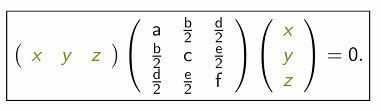
\includegraphics{./figures/L2.1}
\end{figure}

and this is just the Hessian of the conic.
 \begin{nlemma}[]
   The conic $\mathcal{C}$ is irreducible if and only if $\det M \ne 0$.
 \end{nlemma}

\begin{eg}
  The conic $xy - z^2 = 0$ is irreducible.
\end{eg}

\subsection{Five Points make a conic}
Let $P_i \in \pc$ for $1\le i \le 5$. Suppose no four points is collinear.

\begin{nthm}[]
  There is a unique conic in $\pc$ that contains these points
\end{nthm}

\begin{proof}[]
  Write down the coordinates of the points, every two points can be cooked up a line, then check three points. Find complex numbers such that,
  \begin{figure}[!ht]
  \centering
  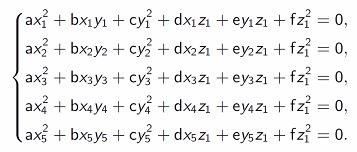
\includegraphics{./figures/L2.2}
  \caption{}
  \end{figure}
These are linear, apply rank-nullity and then it's dimension is not zero. Find null space, so there is at least one conic. Next proof that the rank is not larger than five, or is exactly five.
\end{proof}

\subsubsection{How to find a conic?}
It would be time consuming by hand, so do it with Python. We can plot the real part of the curve as just curves.

\subsubsection{Intersection of line and a conic}
Let $L$ be a line in $\pc$. Let $C$ be an irreducible conic in $\pc$

\begin{nlemma}[]
  The intersection of $L \cap C$ consists of 2 points.
\end{nlemma}

\begin{proof}[]
  The $L$ is given by,
  $$ \a x + \b y + \g z = 0 $$
  for $\a, \b, \g \in \C$ such that they are non-zero. The conic $C$ is given by,
  $$ ax^2 + bxy + cy^2 + dxz + eyz + fz^2 = 0 $$
  for $a, b, c, d, e, f \in \C$ such that ... . Then $L \cup C$ is,
  $$ \begin{cases}
    \a x + \b y + \g z = 0 \\
    ax^2 + bxy + cy^2 + dxz + eyz + fz^2 = 0
  \end{cases} $$
  which then has solutions, which are 2 as we have a quadratic.
\end{proof}

If we consider, an example.
\begin{eg}
  $L : 2x + 7y - 5z = 0$ and $C : 2x^2 -3xy + 7y^2 - 5xz + 11yz - 8z^2$. Firstly we check at infinity. The intersection of $L_z \cap L \cap \mathcal{C}$ and see this is empty, then look at non-infinity, by letting $z = 1$, and substitute and get quadratic equations and get two numbers. If discriminant is negative, this isn't a problem as we are algebraically closed.
\end{eg}

Let $L$ be a line in $\pc$, and let $\mathcal{C}$ be irreducible in $\pc$.

\begin{question}
  When $|L \cap \mathcal{C}| = 1$?
\end{question}

If we consider finite fields, our pictures are intuitive, but we can still study tangents. We may assume $[0:0:1] \in L \cap \mathcal{C}$. Then $\mathcal{C}$ is given by,
$$ \mathbf{a}x^2 + \mathbf{b}xy + \mathbf{c}y^2 + \mathbf{d}xz + \mathbf{e}yz = 0 $$
for some $[\mathbf{a} : \mathbf{b} : \mathbf{c} : \mathbf{d}] \in \P_\C^4$.\\
we may assume that $L$ is given by $x=0$. Then,
$$ L\cap \mathcal{C} = [0 : 0 : 1] \cup [0 : \mathbf{e} : -\mathbf{c}] $$
and so we have $|L \cap \mathcal{C}| 0 \iff \mathbf{e} = 0$.\\

\begin{itemize}
  \item Let $U_z$ be the complement in $\pc$ to the line $z = 0$
  \item Identify $U_z = \C^2$ with coordinates $\overline x = \frac{x}{z}$ and $\overline y = \frac{y}{z}$
\end{itemize}
Then $U_z \cap \mathcal{C}$ is given by $\mathbf{a}\overline x^2$

\begin{figure}[!ht]
\centering
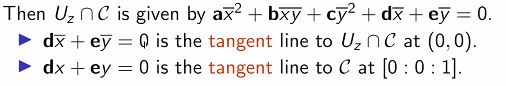
\includegraphics{./figures/L2.3}
\end{figure}

Then $|L \cap \mathcal{C}| = 1 \iff$ $L$ is tangent to $\mathcal{C}$ at point $L \cap \mathcal{C}$

\subsection{Conics and projective transformations}
Let $\mathcal{C}$ be a conic,
\begin{nthm}[]
  There is projective transformations $\phi$ such that $\phi(\mathcal{C})$ is given by,
  \begin{enumerate}
    \item either $xy = z^2$ (irreducible smooth conic)
    \item $xy = 0$ (a union of two lines in $\pc$)
    \item $x^2 = 0$ (a line in $\pc$ taken with multiplicity 2)
  \end{enumerate}
\end{nthm}
The proof could use Grahm Schmitz Orthogonalisation.\footnote{This is course is made acessible ;)} We can instead do group thory by studing an 8 dimensional group. We will then quotient this with three orbit (one normal, two special (unstable)).

\begin{itemize}
  \item Pick a point in $\mathcal{C}$ and map it to $[0 : 0 : 1]$. This {\color{blue} kills }$f$.
  \item Map the tangent line $dx + ey = 0$ to $x = 0$. This {\color{orange} kills }$e$.
  \item Map the line $z = 0$ to the line,
  $$ z + \a y + \b z $$
  for appropriate $\a, \b$ to {\color{green} kills} $a$ and $b$
  \item Scale $x, y$ and $z$ to get $b = 1$ and $c = - 1$
\end{itemize}
This gives a projective Classification, i.e. the conic is just
$$ xy = z^2 $$

\subsection{Intersecting Two Conics}

\begin{nthm}[]
  The intresection of $\mathcal{C} \cap \mathcal{C}'$ consists one one, two or three or four points.
\end{nthm}

\begin{proof}[]
  We can use Classification theorem, so just go to $xy = z^2$.
  \begin{itemize}
    \item Let $L$ be the line $y = 0$. Then $L cap \mathcal{C} \cap \mathcal{C}' \subset [1 : 0 : 0]$
    \item One has $L \cap \mathcal{C} \cap \mathcal{C}' = [1 : 0 : 0] \iff a = 0 $
    \item Let $U$
  \end{itemize}
  \begin{figure}[!ht]
  \centering
  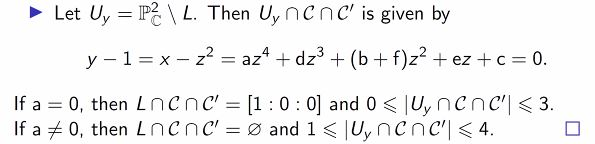
\includegraphics{./figures/L2.4}
  \caption{}
  \end{figure}
\end{proof}

Here are some examples of

\end{document}
